\documentclass[12pt,a4paper]{scrartcl}
\usepackage[utf8]{inputenc}
\usepackage[english,russian]{babel}
\usepackage{indentfirst}
\usepackage{misccorr}
\usepackage{graphicx}
\usepackage{amsmath}
\usepackage{graphics}

\begin{document}
	\begin{center}	
		Алгоритмы и структуры данных. Семинар 25.
		Графы, задачи интересные и не очень. \\
		Григорьев Дмитрий БПМИ-163\\
	\end{center}
	\textbf{Задача 1.} \\
	Рассмотрим самый длинный простой путь, то есть такой путь, в котором вершины не повторяются, т. к. $k$ $\geqslant 2$, то длина этого пути $\geqslant 3$: \\
	$v_1$ -- $v_2$ -- $\cdot \cdot \cdot$ -- $v_r$\\
	Вершина $v_1$ имеет степень не менее 2, поэтому она соединена с еще 2 вершинами. Если какая то из этих вершин отлична от вершин с самого длиного простого пути (	$v_1$ -- $v_2$ -- $\cdot \cdot \cdot$ -- $v_r$), то мы бы могли удлиннить этот путь, следовательно вершины, с которыми соединена $v_1$ находятся на этом пути.\\
	Пусть $j > 1$ -- максимальный из таких номеров, для которого $v_1$ соединена с $v_j$. При этом возникает простой цикл длиной $j$.\\
	Соединений у вершины $v_1$ может быть не более $j - 1$: только с вершинами $v_2$, ... , $v_j$. Следовательно, $d \leq j - 1$, то есть длина цикла $j \geq d + 1$.	\\
	\begin{flushright}
		ч.т.д.
	\end{flushright}
	\textbf{Задача 2.} \\
	Невозможно построить такой граф, если $a < b < a/2$.\\
	А построить этот граф несложно(если $b \geq a/2$):\\
	$\bullet$ Если $a$ -- четно, то сначала построим бамбук длины $a$. И к средней вершине на бамбуке присоединим новый бамбук длины $b - a/2 - 1$ \\
	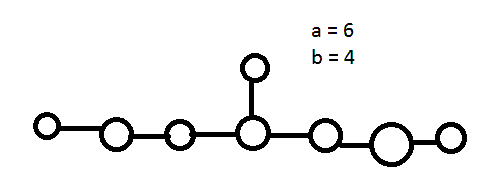
\includegraphics[weight=100, height = 100]{ffff.png}
	\\
	$\bullet$ Если $a$ -- нечетно, то сначала построим бамбук длины $a$. И к средним вершинам на бамбуке присоединим новый бамбук длины $b - a/2 - 1$ \\
	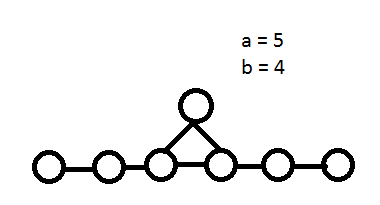
\includegraphics[weight=100, height = 100]{fffff.png}
	\\
	\newpage
	\noindent
	\textbf{Задача 4.} \\
	Рассмотрим данный граф. Если мы начнем с вершины 1, то к концу алгоритма получим, что конец диаметра -- это вершины 1 и 2, а если внимательно посмотреть, то концами диаметра этого графа вершины 3 и 4. 
	
	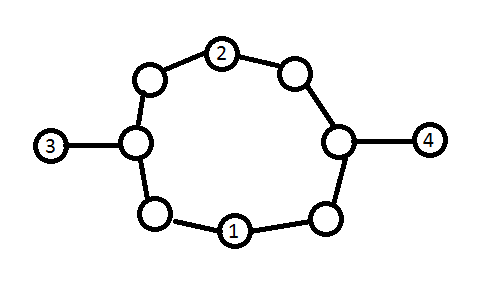
\includegraphics[weight=200, height = 150]{f.png}
	\\
	\textbf{Задача 5.} \\
	Выделим компоненты сильной связности. Решаем для каждой компоненты отдельно. Просто в два цвета красим вершины в каждой компоненте и если для какой--то вершины нашли соединенную с ней такого же цвета, то получили, что имеем цикл нечетно длины. \\
	\\
	\textbf{Задача 6.} \\
	Найдем вершину с наибольшей степенью исходящих ребер -- $v$. Тогда эта вершина и будет ответом, так как если есть вершина, до которой мы не можем дойти сразу из $v$, то мы сможем найти вершину, до которой расстояние из $v$ -- 1, из которой мы можем дойти до остальных, так как при несоблюдении этого $v$ бы не была вершиной с наибольшей степенью исходящих ребер.\\
	\\
	\textbf{Задача 9.} \\
	Для начала удалим все мосты и получим компонеты связности. Сжимаем их. Далее возвращаем назад удаленные мосты. Теперь в полученном дереве найдем диаметр и искомым ребром будет ребро между концами найденого диаметра, так как тогда мы получим минимальное количество мостов.
	
\end{document}
